\documentclass[10pt,tikz,border=0pt]{standalone}
\usepackage[T1]{fontenc}
\usepackage[default]{sourcesanspro}
\usepackage{newtxsf}
\usepackage{amssymb}
\usepackage{tikz}
\usetikzlibrary{arrows.meta,positioning,calc,shapes.geometric}

\definecolor{cA}{HTML}{0F766E}
\definecolor{cAbg}{HTML}{ECFDF5}
\definecolor{cB}{HTML}{B45309}
\definecolor{cBbg}{HTML}{FFFBEB}
\definecolor{cGit}{HTML}{4338CA}
\definecolor{cDet}{HTML}{334155}
\definecolor{cDetbg}{HTML}{F1F5F9}
\definecolor{cHum}{HTML}{BE123C}
\definecolor{cHumbg}{HTML}{FFF1F2}
\definecolor{ink}{HTML}{0F172A}
\definecolor{mid}{HTML}{5A6577}
\definecolor{faint}{HTML}{9AA4B2}
\definecolor{hair}{HTML}{D8DEE7}
\definecolor{band}{HTML}{1E2A55}

\newcommand{\kick}[2]{{\scriptsize\bfseries\color{#1}#2}}
\newcommand{\hl}[1]{{\small\bfseries\color{band}#1}}
\newcommand{\lb}[1]{{\scriptsize #1}}
\newcommand{\fpt}[1]{{\tiny\color{mid}#1}}

\begin{document}
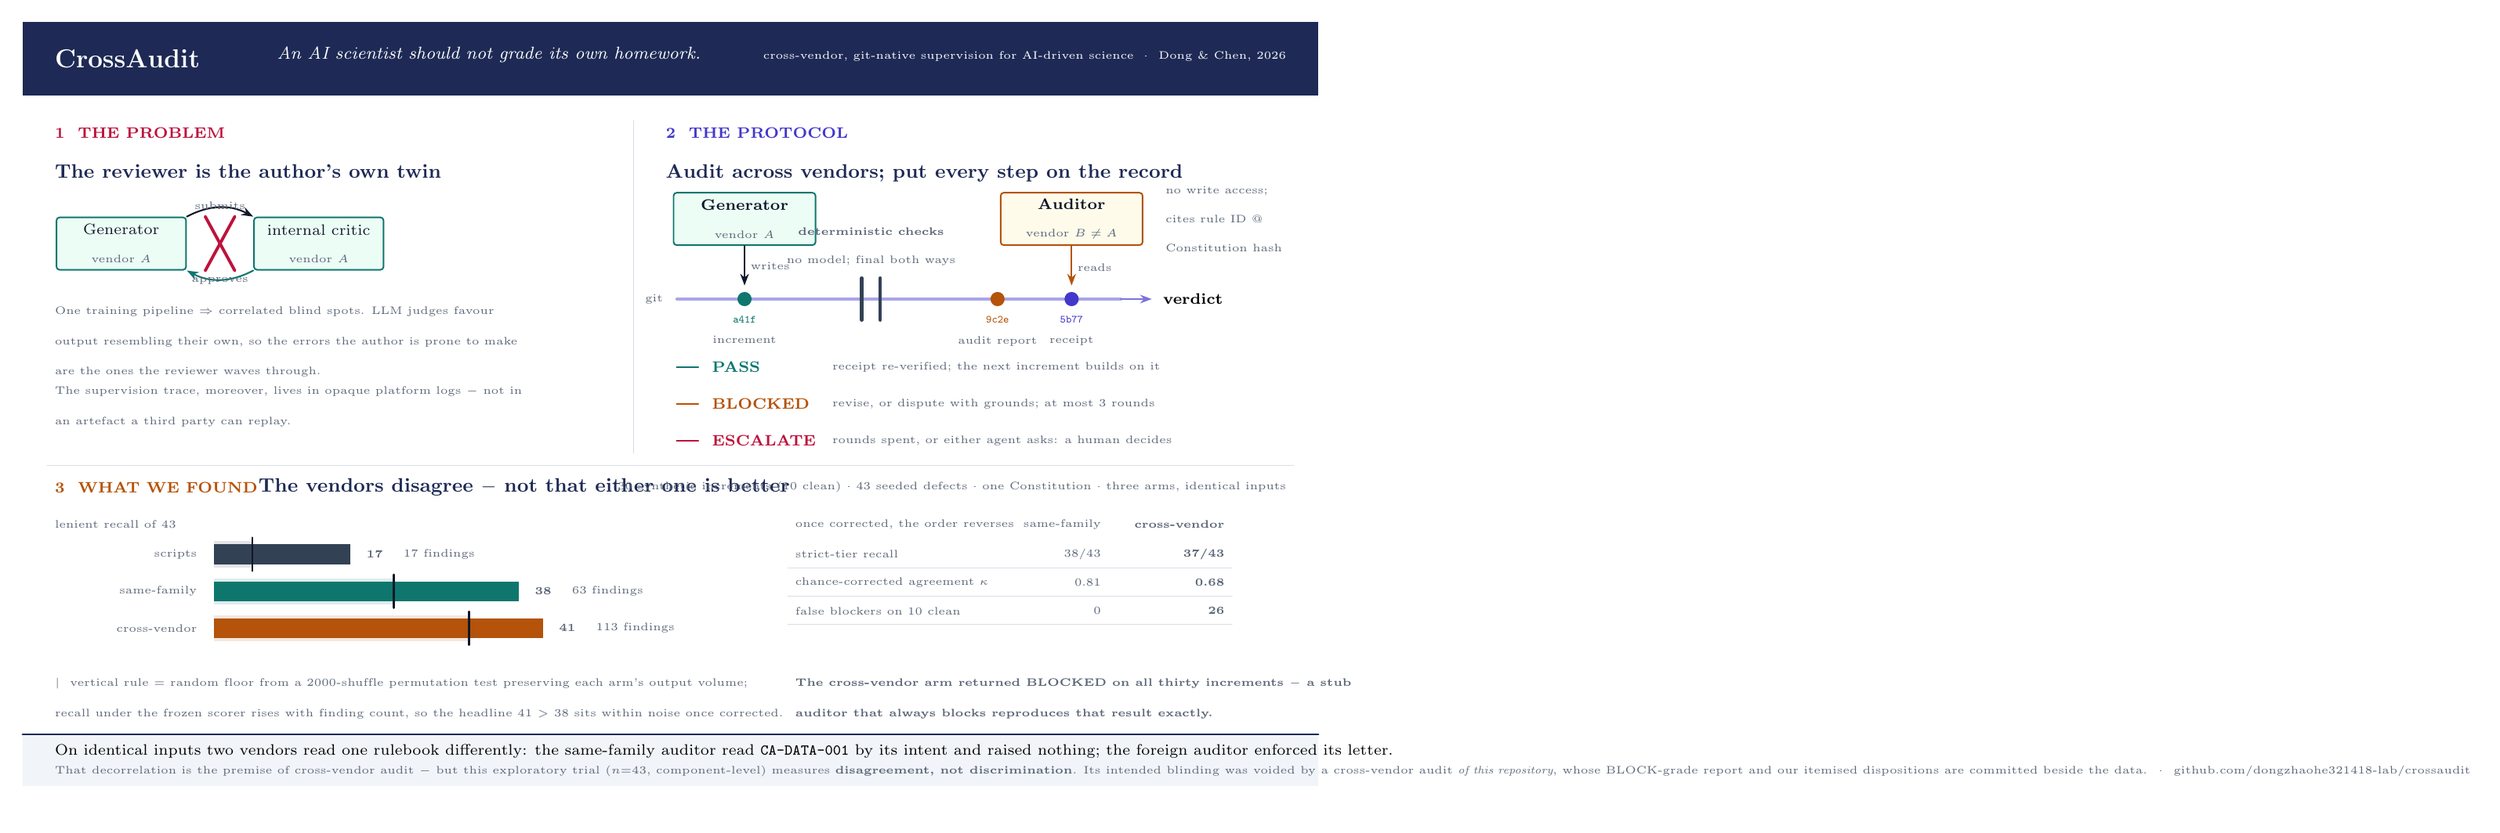
\begin{tikzpicture}[x=1mm,y=1mm,line join=round,line cap=round,
  every node/.append style={execute at begin node=\hyphenpenalty10000\exhyphenpenalty10000\relax}]
\tikzset{
  box/.style={rounded corners=1.4pt,line width=.7pt,align=center,inner sep=2.4pt},
  ar/.style={-{Stealth[length=1.9mm,width=1.4mm]},line width=.75pt,color=ink},
  hairline/.style={line width=.45pt,color=hair},
  dot/.style={circle,inner sep=0pt,minimum size=2.3mm},
  fpn/.style={font=\tiny,text=mid,inner sep=1pt},
}
\path (0,-4) rectangle (210,124);

% ================== HEADER ==================
\fill[band] (0,112) rectangle (210,124);
\node[anchor=west,text=white] at (4,118) {\large\bfseries CrossAudit};
\node[anchor=west,text=white!88] at (40,118.6)
   {\footnotesize\itshape An AI scientist should not grade its own homework.};
\node[anchor=east,text=white!62] at (206,118.4)
   {\tiny cross-vendor, git-native supervision for AI-driven science \ \textperiodcentered\ \ Dong \& Chen, 2026};

% ================== ACT 1 (left column) ==================
\node[anchor=west] at (4,106) {\kick{cHum}{1\ \ THE PROBLEM}};
\node[anchor=north west] at (4,102) {\hl{The reviewer is the author's own twin}};

\node[box,draw=cA,fill=cAbg,text=ink,minimum width=21mm,minimum height=8.5mm] (t1) at (16,88)
   {\lb{Generator}\\[.3mm]\fpt{vendor $A$}};
\node[box,draw=cA,fill=cAbg,text=ink,minimum width=21mm,minimum height=8.5mm] (t2) at (48,88)
   {\lb{internal critic}\\[.3mm]\fpt{vendor $A$}};
\draw[ar] (t1.north east) to[out=28,in=152] node[fpn,pos=.5,above=-.8mm]{submits} (t2.north west);
\draw[ar,color=cA] (t2.south west) to[out=-152,in=-28] node[fpn,pos=.5,below=-.8mm]{approves} (t1.south east);
\draw[line width=1.4pt,color=cHum] (29.6,92.4) -- (34.4,83.6);
\draw[line width=1.4pt,color=cHum] (34.4,92.4) -- (29.6,83.6);

\node[anchor=north west,align=left] at (4,79)
  {\fpt{One training pipeline $\Rightarrow$ correlated blind spots. LLM judges favour}\\[.7mm]
   \fpt{output resembling their own, so the errors the author is prone to make}\\[.7mm]
   \fpt{are the ones the reviewer waves through.}};
\node[anchor=north west,align=left] at (4,66)
  {\fpt{The supervision trace, moreover, lives in opaque platform logs $-$ not in}\\[.7mm]
   \fpt{an artefact a third party can replay.}};

\draw[hairline] (99,54) -- (99,108);

% ================== ACT 2 (right column) ==================
\node[anchor=west] at (103,106) {\kick{cGit}{2\ \ THE PROTOCOL}};
\node[anchor=north west] at (103,102) {\hl{Audit across vendors; put every step on the record}};

\node[box,draw=cA,fill=cAbg,text=ink,minimum width=23mm,minimum height=8.5mm] (gen) at (117,92)
   {\lb{\bfseries Generator}\\[.3mm]\fpt{vendor $A$}};
\node[box,draw=cB,fill=cBbg,text=ink,minimum width=23mm,minimum height=8.5mm] (aud) at (170,92)
   {\lb{\bfseries Auditor}\\[.3mm]\fpt{vendor $B \neq A$}};
\node[anchor=west,align=left] at (184,92)
   {\fpt{no write access;}\\[.5mm]\fpt{cites rule ID @}\\[.5mm]\fpt{Constitution hash}};

\draw[ar] (gen.south) -- (117,81.2) node[fpn,pos=.5,right=.5mm]{writes};
\draw[ar,color=cB] (170,87.8) -- (170,81.2) node[fpn,pos=.55,right=.5mm]{reads};

% git spine
\draw[line width=1.15pt,color=cGit!45] (106,79) -- (178,79);
\node[anchor=east,text=cGit] at (105,79) {\fpt{git}};
\foreach \x/\c/\h/\l in {117/cA/{a41f}/{increment}, 158/cB/{9c2e}/{audit report}, 170/cGit/{5b77}/{receipt}}
  {\node[dot,fill=\c] at (\x,79) {};
   \node[anchor=north] at (\x,77.4) {{\tiny\ttfamily\bfseries\color{\c}\h}};
   \node[anchor=north] at (\x,74.2) {\fpt{\l}};}

% deterministic gate: a real gate glyph on the spine
\draw[line width=1.6pt,color=cDet] (136,82.4) -- (136,75.6);
\draw[line width=1.6pt,color=cDet] (139,82.4) -- (139,75.6);
\node[anchor=south,align=center] at (137.5,83.2) {\fpt{\bfseries deterministic checks}\\[.3mm]\fpt{no model; final both ways}};

\draw[ar,color=cGit!70] (178,79) -- (183,79);
\node[anchor=west] at (183.6,79) {\lb{\bfseries verdict}};

\foreach \y/\c/\t/\d in {%
   68/cA/{PASS}/{receipt re-verified; the next increment builds on it},
   62/cB/{BLOCKED}/{revise, or dispute with grounds; at most 3 rounds},
   56/cHum/{ESCALATE}/{rounds spent, or either agent asks: a human decides}}
{
  \draw[line width=.8pt,color=\c] (106,\y) -- (109.5,\y);
  \node[anchor=west,text=\c] at (110.5,\y) {\lb{\bfseries\t}};
  \node[anchor=west] at (130,\y) {\fpt{\d}};
}

% ================== ACT 3 (full-width band) ==================
\draw[hairline] (4,52) -- (206,52);
\node[anchor=west] at (4,48.4) {\kick{cB}{3\ \ WHAT WE FOUND}};
\node[anchor=west] at (37,48.5) {\hl{The vendors disagree $-$ not that either one is better}};
\node[anchor=east] at (206,48.5)
   {\fpt{30 synthetic increments (10 clean) \textperiodcentered\ 43 seeded defects \textperiodcentered\ one Constitution \textperiodcentered\ three arms, identical inputs}};

% ---- bars ----
\def\bx{31}
\def\bs{1.30}
\node[anchor=west,text=mid] at (4,42.4) {\fpt{lenient recall of 43}};
\foreach \y/\c/\nm/\v/\f/\n in {%
   37.6/cDet/{scripts}/{17}/{4.8}/{17},
   31.6/cA/{same-family}/{38}/{22.4}/{63},
   25.6/cB/{cross-vendor}/{41}/{31.8}/{113}}
{
  \node[anchor=east,text=ink] at (\bx-1.5,\y) {\fpt{\nm}};
  \fill[\c!14] (\bx,\y-2.1) rectangle (\bx+\f*\bs,\y+2.1);
  \fill[\c] (\bx,\y-1.6) rectangle (\bx+\v*\bs,\y+1.6);
  \draw[line width=1pt,color=ink] (\bx+\f*\bs,\y-2.7) -- (\bx+\f*\bs,\y+2.7);
  \node[anchor=west,text=ink] at (\bx+\v*\bs+1.4,\y) {\fpt{\bfseries\v}};
  \node[anchor=west,text=faint] at (\bx+\v*\bs+7,\y) {\fpt{\,\n\ findings}};
}
\node[anchor=south west,align=left] at (4,9.6)
  {\fpt{\textbar\ \ vertical rule $=$ random floor from a 2000-shuffle permutation test preserving each arm's output volume;}\\[.8mm]
   \fpt{recall under the frozen scorer rises with finding count, so the headline 41 $>$ 38 sits within noise once corrected.}};

% ---- the reversal table ----
\def\tx{124}
\node[anchor=west,text=mid] at (\tx,42.4) {\fpt{once corrected, the order reverses}};
\node[anchor=east,text=cA] at (\tx+52,42.4) {\fpt{same-family}};
\node[anchor=east,text=cB] at (\tx+72,42.4) {\fpt{\bfseries cross-vendor}};
\foreach \i/\nm/\a/\b in {0/{strict-tier recall}/{38/43}/{37/43},
                          1/{chance-corrected agreement $\kappa$}/{0.81}/{0.68},
                          2/{false blockers on 10 clean}/{0}/{26}}
{
  \node[anchor=west,text=mid] at (\tx,37.6-\i*4.6) {\fpt{\nm}};
  \node[anchor=east,text=cA]  at (\tx+52,37.6-\i*4.6) {\fpt{\a}};
  \node[anchor=east,text=cB]  at (\tx+72,37.6-\i*4.6) {\fpt{\bfseries\b}};
  \draw[hairline] (\tx,35.4-\i*4.6) -- (\tx+72,35.4-\i*4.6);
}
\node[anchor=south west,align=left,text=cHum] at (\tx,9.6)
  {\fpt{\bfseries The cross-vendor arm returned BLOCKED on all thirty increments $-$ a stub}\\[.8mm]
   \fpt{\bfseries auditor that always blocks reproduces that result exactly.}};

% ================== PUNCHLINE ==================
\fill[cDetbg] (0,0) rectangle (210,8.4);
\draw[line width=.8pt,color=band] (0,8.4) -- (210,8.4);
\node[anchor=west,align=left] at (4,5.6)
  {\lb{On identical inputs two vendors read one rulebook differently: the same-family auditor read \texttt{CA-DATA-001} by its intent and raised nothing; the foreign auditor enforced its letter.}};
\node[anchor=west,align=left] at (4,2.4)
  {\fpt{That decorrelation is the premise of cross-vendor audit $-$ but this exploratory trial ($n{=}43$, component-level) measures \textbf{disagreement, not discrimination}. Its intended blinding was voided by a cross-vendor audit \emph{of this repository}, whose BLOCK-grade report and our itemised dispositions are committed beside the data. \ \textperiodcentered\ \ github.com/dongzhaohe321418-lab/crossaudit}};
\end{tikzpicture}
\end{document}
